\chapter{Time Tracking Report}

\instructions{
    \section{How we track time}
    We record and plan all our tasks with individual issues on Gitlab.

    For every task we estimate how much time it is going to take. Then, every team member reports their time spent on that task.
    The estimated and spent times are tracked with an accuracy of 15 minutes.

    \section{Time tracking statistics}
    8 hours count as 1 day in this context. Detailed reports for every milestone can be found on our repository\footnote{\url{https://gitlab.ost.ch/SEProj/2022-FS/g03-kubewatch/kubewatch/-/tree/main/Documentation/time-tracking}}. Milestone reports are in Markdown (.md) and start with the corresponding milestone number (M1, M2, ...).

    \subsection{Milestone 1: Project Plan}
    \begin{itemize}
        \item Total estimate: 6d 2h 45m
        \item Total spent: 5d 4h 45m
        \item The detailed report can be found \href{https://gitlab.ost.ch/SEProj/2022-FS/g03-kubewatch/kubewatch/-/blob/main/Documentation/time-tracking/M1\%20Project\%20Plan\%20Time\%20Tracking\%20Report.md}{here}.
    \end{itemize}
    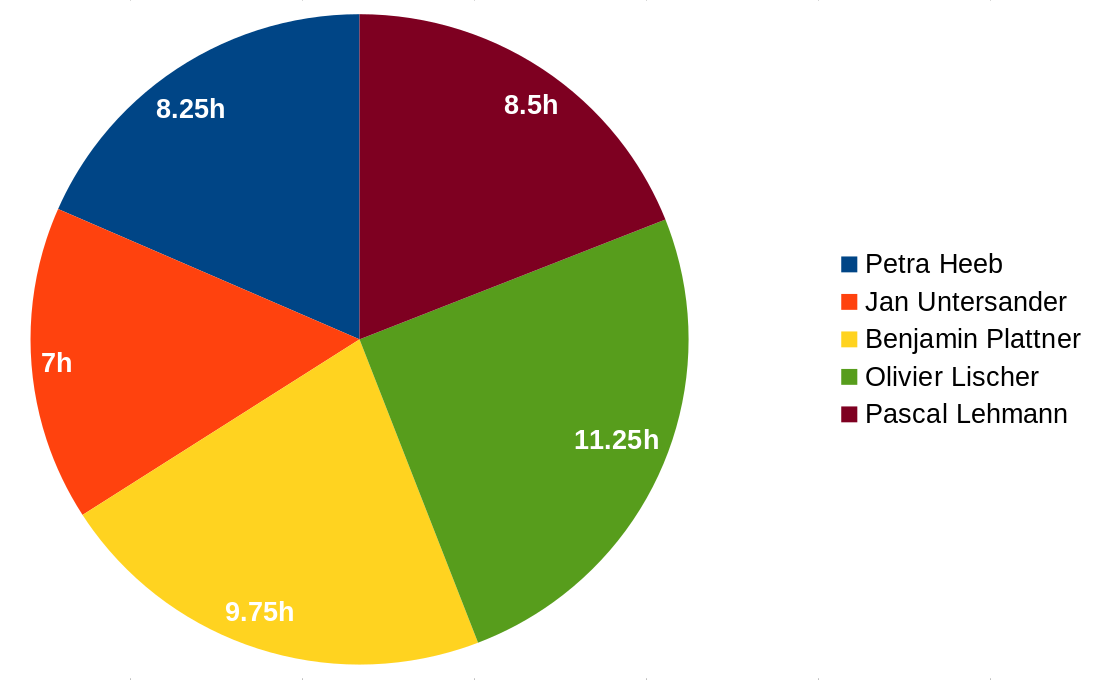
\includegraphics[width=12cm]{resources/m1_time_tracking_chart.png}

    \subsection{Milestone 2: Requirements}
    \begin{itemize}
        \item Total estimate: 8d 1h
        \item Total spent: 8d 6h 10m
        \item The detailed report can be found \href{https://gitlab.ost.ch/SEProj/2022-FS/g03-kubewatch/kubewatch/-/blob/main/Documentation/time-tracking/M2\%20Requirements\%20Time\%20Tracking\%20Report.md}{here}.
    \end{itemize}
    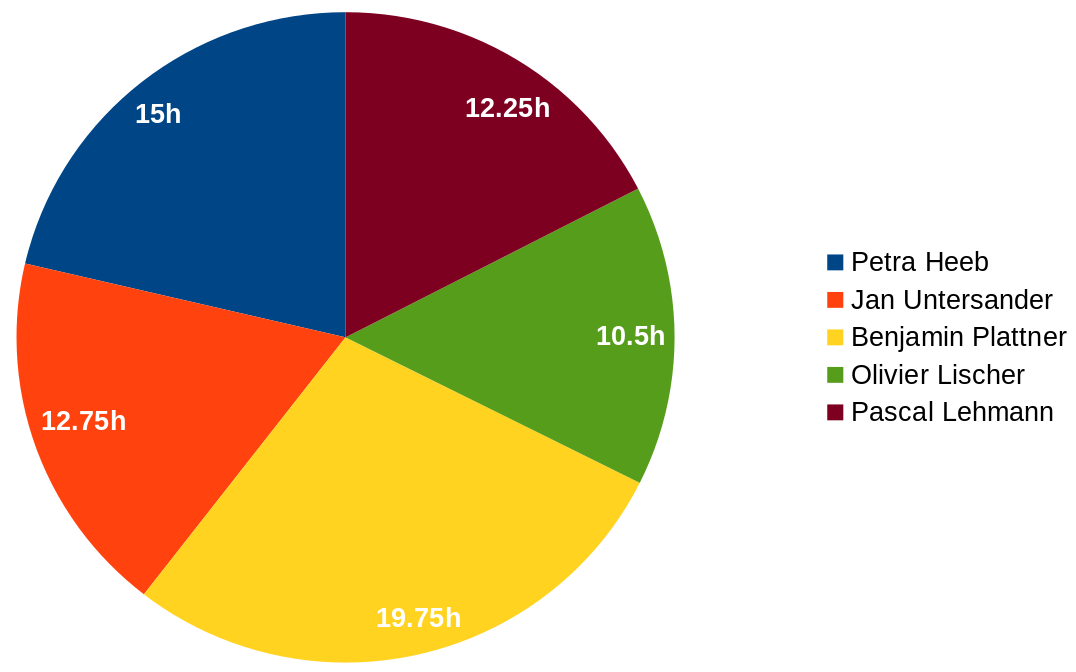
\includegraphics[width=12cm]{resources/m2_time_tracking_chart.png}
}